\section{Recall rises from $S_1{=}2$ to $S_1{=}6$, but no budget matches dense}
\label{sec:budget}

We first trace recall against $S_1$ on the pilot seed, then test chosen settings on three untouched seeds against
dense attention trained on identical data. All results in this section use the M5 profile (TF32, isolated data;
\S\ref{sec:setup}), and $K{=}4$ throughout.

\subsection{The pilot curve}

Table~\ref{tab:budget} and Figure~\ref{fig:budget}a show held-out recall at the four settings on seed 123. Recall rose
from 0.705 at $S_1{=}2$ (34 selector scores per query) to 0.884 at $S_1{=}4$ (56) and 0.962 at $S_1{=}6$ (78).
$S_1{=}12$ scored 0.850. At $L{=}2048$ there are 12 super-blocks, so $S_1{=}12$ keeps them all: its fine level chooses
the top 4 among all eligible blocks, which is flat block selection plus a redundant parent pass. On this one seed, the
hierarchical setting $S_1{=}6$ therefore beat effectively flat selection; one run per point cannot establish the order.
The two further pilot seeds at $S_1{=}2$ scored 0.684 and 0.836, a range of 0.152 at the cheapest setting.

\begin{table}[t]
\centering
\small
\begin{tabular}{lrrrr}
\toprule
Setting & selector scores / query & held-out recall & best validation (epoch) & transition epoch \\
\midrule
$S_1{=}2$  & 34  & 0.705 & 0.704 (53) & 41 \\
$S_1{=}4$  & 56  & 0.884 & 0.885 (59) & 34 \\
$S_1{=}6$  & 78  & 0.962 & 0.962 (58) & 29 \\
$S_1{=}12$ (flat) & 144 & 0.850 & 0.850 (37) & 26 \\
dense      & -- & 0.010 & 0.010 (55) & never \\
\bottomrule
\end{tabular}
\caption{\textbf{On the pilot seed, recall rises from $S_1{=}2$ to $S_1{=}6$ and falls at $S_1{=}12$.} Seed 123,
$L{=}2048$, $K{=}4$, M5 profile, one run per row. Selector scores per query are a count, not runtime. $S_1{=}12$ keeps
all 12 super-blocks, which makes it effectively flat selection. Dense did not transition on this seed within 60
epochs (\S\ref{sec:dense}).}
\label{tab:budget}
\end{table}

\subsection{What the $S_1$ axis measures on this task}

Every key in this MQAR layout lies in the first 256 tokens, inside super-blocks 0 and 1. A selector that always kept
those two super-blocks would lose no key at $S_1{=}2$, so pruning at the parent level need not discard any needed
information. What does change with $S_1$ is the fine level's candidate set: 22 blocks at $S_1{=}2$, 66 at $S_1{=}6$ and all 128 real blocks at $S_1{=}12$, of which at most 16 hold keys. A larger set nominally makes the fine choice harder, yet recall rose
up to $S_1{=}6$. We therefore read the curve as a measure of how reliably the selector learns to choose at fixed $K$,
not of information that pruning throws away. Section~\ref{sec:selection} shows what changes in the trained models: at $S_1{=}2$ they still
miss the key's super-block on 5--14\% of queries, and from $S_1{=}4$ up they do not.

\subsection{On untouched seeds, $S_1{=}6$ beats $S_1{=}2$ every time but stays below dense}

Before any M5 data we reserved seeds 810001--810003 and pre-registered a rule for which setting to confirm on them:
the smallest $S_1$ whose pilot validation recall came within 0.02 of dense's, with a hold for the owner if dense or a
pilot run \emph{failed}. Dense completed all 60 epochs without transitioning; we did not treat that as a failure, so
every setting qualified and the rule chose $S_1{=}2$ vacuously. This reading of the hold clause was ours, made before
the confirmation runs. We ran dense and $S_1{=}2$ on all three seeds, and then, under a second pre-registration written
after the pilot, $S_1{=}6$ on all three (Table~\ref{tab:reserved}, Figure~\ref{fig:budget}b). Within a seed every
model trained and was tested on byte-identical splits, verified by SHA-256 hashes in the run manifests.

\begin{table}[t]
\centering
\small
\begin{tabular}{rrrrrr}
\toprule
Seed & dense & $S_1{=}2$ & $S_1{=}6$ & $S_1{=}6 - S_1{=}2$ & dense $-$ $S_1{=}6$ \\
\midrule
123 (pilot) & 0.010$^\dagger$ & 0.705 & 0.962 & $+0.257$ & n/a \\
810001 & 0.012$^\dagger$ & 0.578 & 0.937 & $+0.359$ & n/a \\
810002 & \textbf{1.000} & 0.709 & 0.945 & $+0.236$ & \textbf{0.055} \\
810003 & 0.006$^\dagger$ & 0.011$^\dagger$ & 0.945 & n/a & n/a \\
\bottomrule
\end{tabular}
\caption{\textbf{Paired on identical data, $S_1{=}6$ beat $S_1{=}2$ on every seed; where dense learned, it beat
both.} Held-out recall; identical data within a seed. On seed 810002, dense $-$ $S_1{=}2$ is 0.291. $^\dagger$No
transition within 60 epochs; gaps to a model that did not learn are not reported. Dense reruns in float32 on 123,
810001 and 810003 are in \S\ref{sec:dense}. $S_1{=}6$ was chosen after the pilot, so its reserved-seed runs confirm a
selected point.}
\label{tab:reserved}
\end{table}

The most robust result is the paired comparison: on all four seeds where both were run, $S_1{=}6$ beat $S_1{=}2$, by
0.236 to 0.359 on the three seeds where both learned; on 810003 $S_1{=}6$ reached 0.945 while $S_1{=}2$ never learned
(Table~\ref{tab:reserved}). $S_1{=}6$ transitioned on all four and was stable across the reserved
seeds (0.937, 0.945, 0.945; standard deviation 0.005), while $S_1{=}2$ failed to transition on 810003.

Only seed 810002 gives a valid dense comparison, because dense did not transition on 810001 or 810003. There, dense
beat $S_1{=}2$ by 0.291 and $S_1{=}6$ by 0.055. Our pre-registered criterion for ``near-dense'' was held-out recall
within 0.02 of a transitioned dense model on the same seed; \textbf{no setting met it}. As unpaired context only: the
other dense run that learned on the isolated data (float32, seed 123) also reached 1.000, and every $S_1{=}6$ run
scored 0.937--0.962.

\begin{figure}[t]
\centering
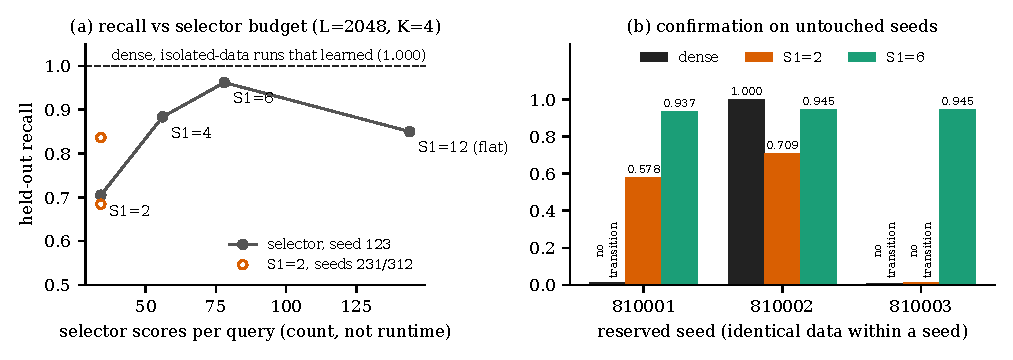
\includegraphics[width=\linewidth]{figures/fig1_budget.pdf}
\caption{\textbf{Recall rises from $S_1{=}2$ to $S_1{=}6$, but no setting matches dense attention where dense
learned.} (a) Held-out recall against selector scores per query on pilot seed 123 (filled), with $S_1{=}2$ on pilot
seeds 231 and 312 (open); $S_1{=}12$ is effectively flat selection. The dashed line marks dense recall on the
isolated-data runs where it transitioned. (b) Held-out recall on three untouched seeds; within a seed all models saw
identical data. ``No transition'' marks runs that never exceeded 0.30 validation recall within 60 epochs.
$L{=}2048$, $K{=}4$, 128 key--value pairs, M5 profile.}
\label{fig:budget}
\end{figure}
